\documentclass[%
a4paper,
twoside,
12pt
]{article}

% encoding, font, language
\usepackage[T1]{fontenc}
\usepackage[utf8]{inputenc}
\usepackage{lmodern}
\usepackage[ngerman]{babel}

\usepackage{nicefrac}
\usepackage{textcomp}
\usepackage{setspace}

\usepackage[
%    handwritten,
    nowarnings,
    %myconfig
]
{config/xcookybooky}



\DeclareRobustCommand{\textcelcius}{\ensuremath{^{\circ}\mathrm{C}}}


\setcounter{secnumdepth}{1}
\renewcommand*{\recipesection}[2][]
{%
    \subsection[#1]{#2}
}
\renewcommand{\subsectionmark}[1]
{% no implementation to display the section name instead
}


\usepackage{hyperref}    % must be the last package
\hypersetup{%
    pdfauthor            = {Kathrin Welzel and Marcel Gro{\ss}mann},
    pdftitle             = {Wedding Recipes},
    pdfsubject           = {Recipes},
    pdfkeywords          = {wedding, recipes, cookbook},
    pdfstartview         = {FitV},
    pdfview              = {FitH},
    pdfpagemode          = {UseNone}, % Options; UseNone, UseOutlines
    bookmarksopen        = {true},
    pdfpagetransition    = {Glitter},
    colorlinks           = {true},
    linkcolor            = {black},
    urlcolor             = {blue},
    citecolor            = {black},
    filecolor            = {black},
}

\hbadness=10000	% Ignore underfull boxes

\begin{document}
\title{Kochbuch anl"asslich der Hochzeit}
\author{Kathrin Welzel \& Marcel Gro{\ss}mann}

\begin{titlepage}
		\setstretch{1.5}
	\centering\fontsize{80pt}{80pt}\fontfamily{pbk}\selectfont

	Kochbuch
	
	\huge
	anl"asslich der Hochzeit
	
	von
	
	\fontsize{40pt}{40pt}\selectfont
	Kathrin \& Marcel
	
	\vfill
	\begin{figure}[h]
		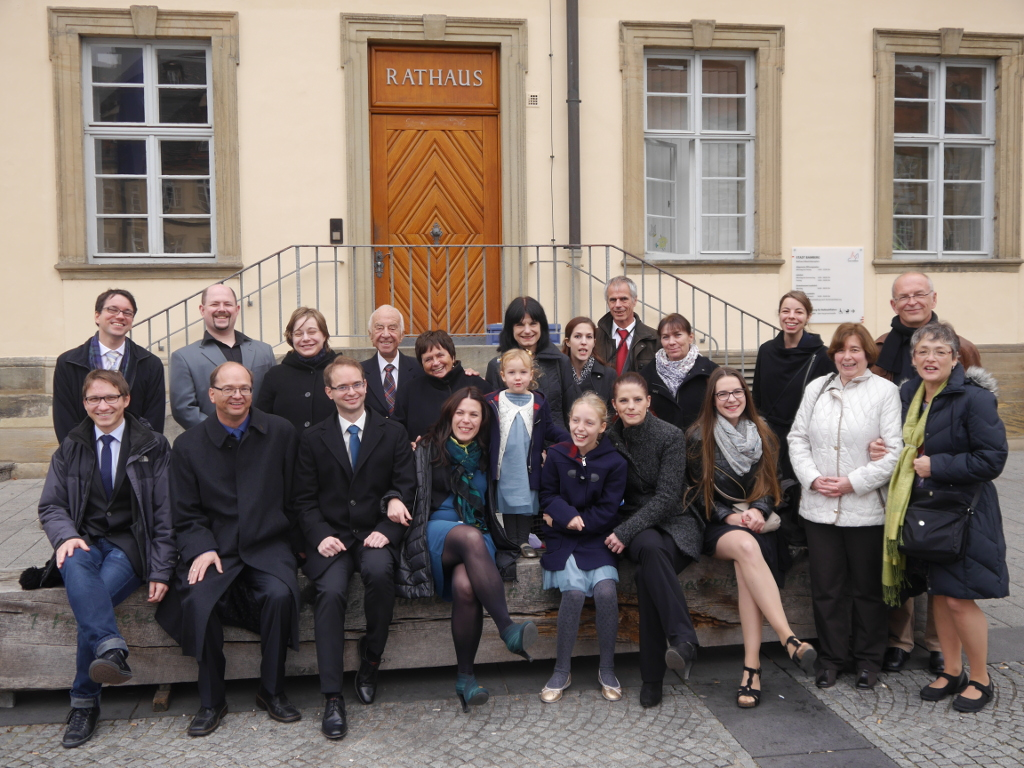
\includegraphics[width=\textwidth]{pic/front.jpg}
	\end{figure}
\LARGE
	\today
\end{titlepage}
\thispagestyle{empty}



\cleardoublepage
\tableofcontents


\cleardoublepage


% background graphic
%\setBackgroundPicture[x, y=-2cm, width=\paperwidth-4cm, height, orientation = pagecenter]{pic/background}

\begin{otherlanguage}{ngerman}
\setHeadlines
{% translation
    inghead = Zutaten,
    prephead = Zubereitung,
    hinthead = Tipp,
    continuationhead = Fortsetzung,
    continuationfoot = Fortsetzung auf n\"achster Seite,
    portionvalue = Personen,
}

%%%%%%%%%%%%%%%%%%%%%%%%%%%%%%%%%%%%%%%%%%%%%%%%%%%%%%%%%%%%%%%%%%%
%				Recipe Section										%
%%%%%%%%%%%%%%%%%%%%%%%%%%%%%%%%%%%%%%%%%%%%%%%%%%%%%%%%%%%%%%%%%%%
\cleardoublepage
\section{Vegetarische Speisen}
\begin{figure}[h]
	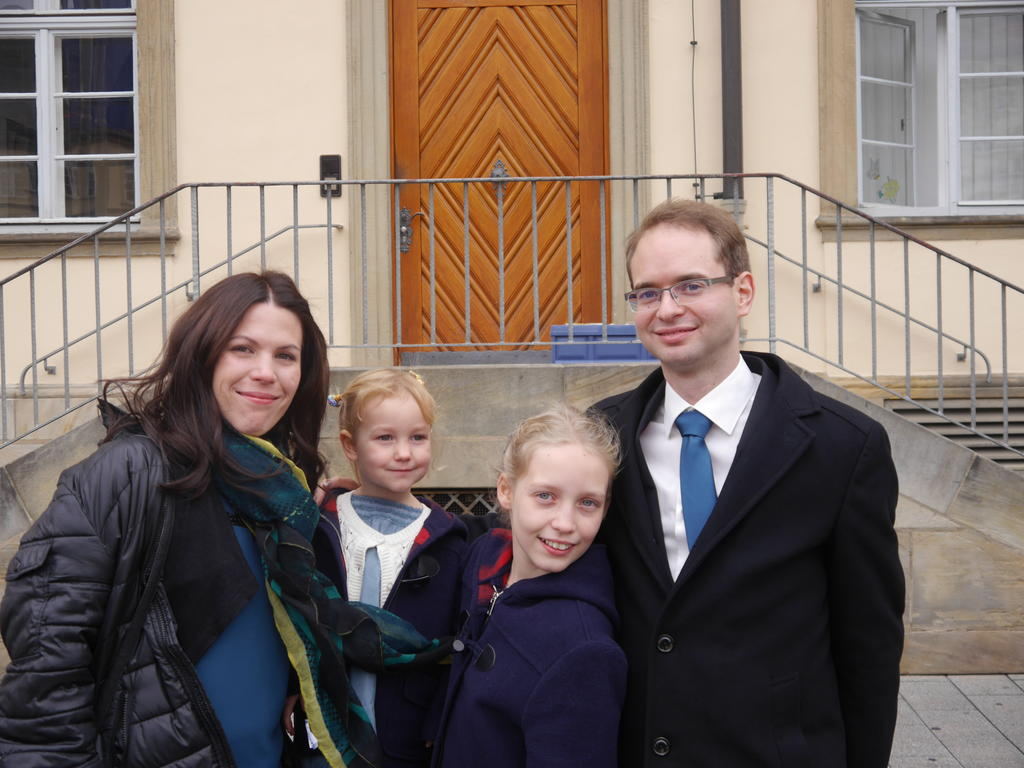
\includegraphics[width=\textwidth]{pic/veggie.jpg}
\end{figure}


\begin{recipe}
[% 
    preparationtime = {\unit[30]{min}},
    portion = {\portion{4}},
    source = {Lieblingsrezept von Ariane (original von chefkoch.de)}
]
{Ratatouille mit Tofu}

    \ingredients{%
        500 g	& 	Tomaten \\
		500 g	& 	Zucchini \\
		500 g &	Paprikaschoten \\
		500 g	&	Aubergine\\
		2	&	Zwiebeln \\
		2	&	Knoblauchzehen \\
		400 g & Räuchertofu \\
		4 EL & Olivenöl\\
		 & Salz und Pfeffer\\
		 2 Stiele & Thymian\\
		2 Stiele & Rosmarin\\
		2 Stiele & Oregano\\
		2 & Lorbeerblatt\\
    }
    
    \preparation{%
    \newline
       \step Das Gemüse gründlich waschen, die Tomaten häuten und in grobe Stücke schneiden. Die Zwiebeln schälen und wie das restliche Gemüse würfeln (ca. erbsengroß). Den Knoblauch schälen und fein hacken. 
       \step Das Olivenöl in einem weiten Topf erhitzen, die Gemüse darin getrennt nach Sorten jeweils 10 Minuten garen, dann herausnehmen (das Gemüse für das Ratatouille getrennt anbraten und erst ganz am Ende miteinander vermischen).
       \step Anschließend den Tofu kurz abtrocknen und würfeln. Das Gemüse vermengen. Die Kräuter mit dem Lorbeerblatt, dem Knoblauch und dem gewürfelten Tofu dazugeben. Mit Salz und Pfeffer würzen und alles weitere 10 Minuten garen.
    }
   
\end{recipe}
% Complete recipe example
\begin{recipe}
% My favourite childhood receipe from my Grandma :)
[%
    preparationtime = {\unit[10]{min}},
    bakingtime={\unit[20]{min}},
    portion = {16--20 pancakes},
    %calory={\unit[3]{kJ}},
    source = {David's favorite Scottish childhood recipe}
]
{Scotch Pancakes (Drop Scones)}

    %\graph
    %{% pictures
        % Unfortunatly I don't have my own picture, but there is an excellent one here: https://www.nigella.com/recipes/scotch-pancakes
    %}

    \ingredients{%
        150 g	         & plain flour \\
                         & pinch of salt \\
        \unitfrac{1}{2} level teasp. & bicarbonate of soda \\
        1 level teasp.   & cream of tartar \\
        1 tablesp.       & caster sugar \\
        1                & beaten egg \\
        1 teasp.         & golden syrup (optional) \\
        120 ml           & milk \\
    }

    \preparation{%
    \newline
       \step Sieve dry ingredients into bowl. Add egg and syrup to mixture. Slowly add milk and beat well to create a batter which will pour from a spoon but must not be too thin. Don't leave standing too long before use.
       \step Heat a heavy frying pan and grease it with lard or white flora. Pour batter on, 1 table spoon at a time (= 1 pancake). Make several at a time but not too close together. When bubbles appear on the surface and just start to burst, turn pancakes over with a palette knife. Cook about 1 minute longer until golden brown.
    }

    \suggestion[Servierbeispiel]
    {%
        Serve with butter and jam.
    }

\end{recipe}

\begin{recipe}
[% 
    preparationtime = {\unit[45]{min}},
    portion = {\portion{2}},
    source = {Ein weiterer Klassiker aus Martins \& Linus' Kochstudio, adaptiert von Chefkoch},
]
{Linus' \& Martins Risotto}
        
    \ingredients{%
		300g	&	Risottoreis\\
		1		& 	Schalotte, klein geschnitten\\
		1 \unitfrac{1}{2} l &	Gem"usebrühe\\
		40g		&	Butter\\
		150ml	&	Weißwein\\
		1 Dose	&	Safranfäden\\
		50g		&	Butter, kalt\\
		150g	&	Parmesan, frisch gerieben\\
				&	Salz\\
				&	Pfeffer
    }
    
    \preparation{%
    \newline
    \step Die Brühe wird in einem Topf heiß gehalten, ohne zu kochen und dann folgt der 1. Schritt, das Anschwitzen -- \textit{solfriggere}. Die Schalotte wird ganz sanft, ohne zu bräunen in 5 Minuten in der Butter angeschwitzt. 
    
    \step Für die 2. Stufe wird der Reis zugegeben und so oft gewendet, bis jedes Korn von der Butter benetzt ist. Dieser Vorgang nennt sich \textit{tostare}. Jetzt wird die Temperatur nach Fingerspitzengefühl leicht erhöht und der Wein angegossen, der ganz verdampfen muss. Nun fügt man den Safran zu. 
    
    \step Schon ist man in der 3. Stufe, dem eigentlichen Kochen, dem \textit{cuocere}, in dem kellenweise die heiße Brühe zugegeben wird. Dieser Vorgang dauert 17 -- 18 Minuten, um einen bissfesten und cremigen Risotto zu kochen. Dabei sollte permanent umgerührt und die Körner vom Rand und Boden des Topfes geschabt werden. 
    
	Die Temperatur muss die Brühe gerade eben kochen lassen und konstant bleiben. Ist die Brühe fast eingekocht, wird die nächste Kelle angegossen. Ab der 14. Minute muss man aufpassen, nicht mehr zu viel Brühe anzugießen, damit der Reis zum Schluss nicht zu flüssig ist. Am Ende des Kochens wird die Hitze deutlich reduziert, um den Reis für 1 Minute ruhen zu lassen. 
    
    \step Dann folgt der 4. und letzte Schritt, die \textit{Mantecatura}, das Verrühren mit kalten Butterwürfeln und frisch geriebenem Parmesan. Nicht vergessen, mit Salz und Pfeffer abzuschmecken. Jetzt sollte die perfekte Konsistenz erreicht sein, die man \textit{Risotto all´onda} nennt. Das bedeutet, wenn man den Topf zur Seite kippt, schlägt der Reis Wellen. 
       
    }
    
    \suggestion[Servierbeispiel]
    {%
		Den Risotto in tiefen Tellern servieren und möglichst bald essen, sonst verliert er seine Konsistenz. Traditionell wird Risotto aber immer ohne Beilagen und erst recht nicht selbst als Beilage gereicht.
    }
    

    \hint{%
       Mehr K"ase ist mehr!
    }
    
\end{recipe}
\begin{recipe}
[% 
    preparationtime = {\unit[30]{min}},
    portion = {\portion{2}},
    source = {Ein Klassiker aus Linus' \& Martins Kochstudio}
]
{Martins \& Linus'  Carbonara}
    

    \ingredients{%
        3 EL	& "Ol \\	
		4       & Eigelb\\
		100g	& Parmesan, frisch gerieben\\
		50g		& Cocktailtomaten\\
				& Muskat\\
				& Salz\\
				& Pfeffer\\
		250g	&  Spaghetti\\
    }
    
    \preparation{%
    \newline
       \step Spaghetti mit reichlich Salz kochen.
       \step W"ahrenddessen die Eigelb mit "Ol und fein geriebenem Parmesan verquirlen. Mit Salz, Pfeffer und Muskat abschmecken.
       \step Cocktailtomaten halbieren.
       \step Spaghettiwasser abgie\ss en und auf der ausgeschalteten Kochstelle mit der Masse so lange vermischen, bis das Eigelb bindet. Nicht zu lange rühren, sonst erhält man ein Rührei. Noch einmal gut mit Salz und Pfeffer w"urzen.
    }
    
    \suggestion[Servierbeispiel]
    {%
		Die Cocktailtomaten kommen roh auf den Teller und geben dem Gericht einen fruchtigen Geschmack.
    }
    

    \hint{%
       Mehr K"ase ist mehr!
    }
    
\end{recipe}

\cleardoublepage
\subsection{Herbstrezepte}
\begin{figure}[h]
	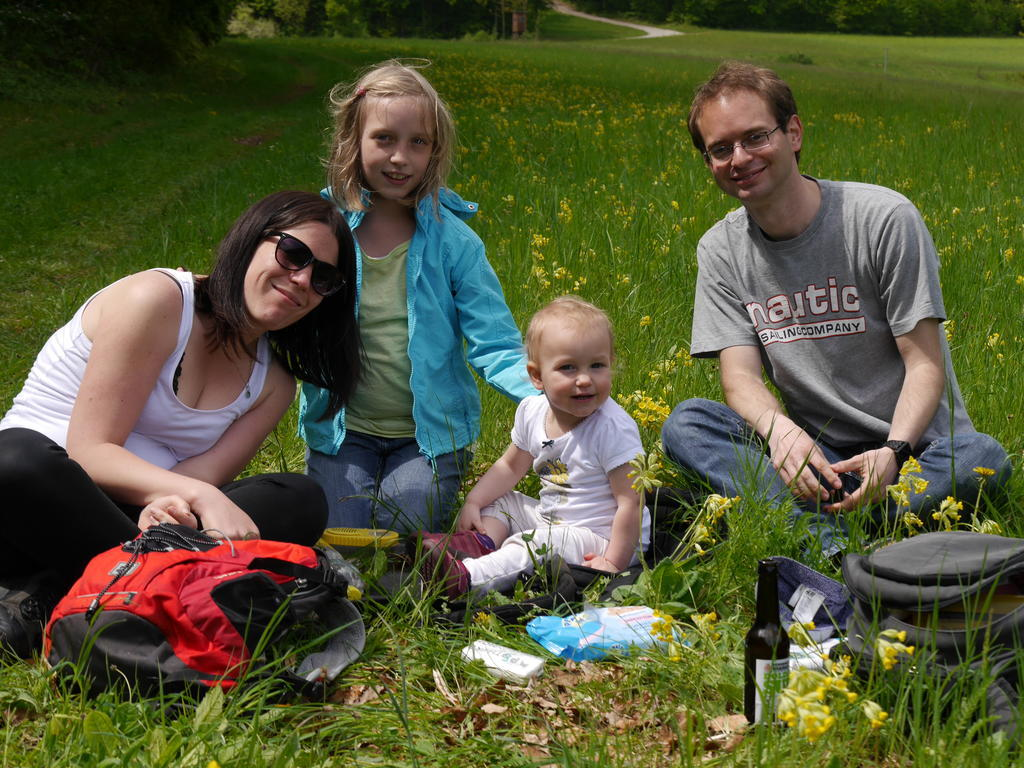
\includegraphics[width=\textwidth]{pic/US}
\end{figure}
\include{recipes/PumpkinSoup}
\include{recipes/CurlyKaleSoup}
\include{recipes/LinsenFenchelEintopf}
\include{recipes/TomatoeBredie}
\include{recipes/BroccoliNoodles}
\include{recipes/MushroomPolenta}
\include{recipes/ColeSlawWok}
\include{recipes/BrokkoliSuesskartoffelAuflauf}
\include{recipes/Cheese}
\include{recipes/AvocadoMouse}

\cleardoublepage
\section{Kuchen}
\begin{figure}[h]
	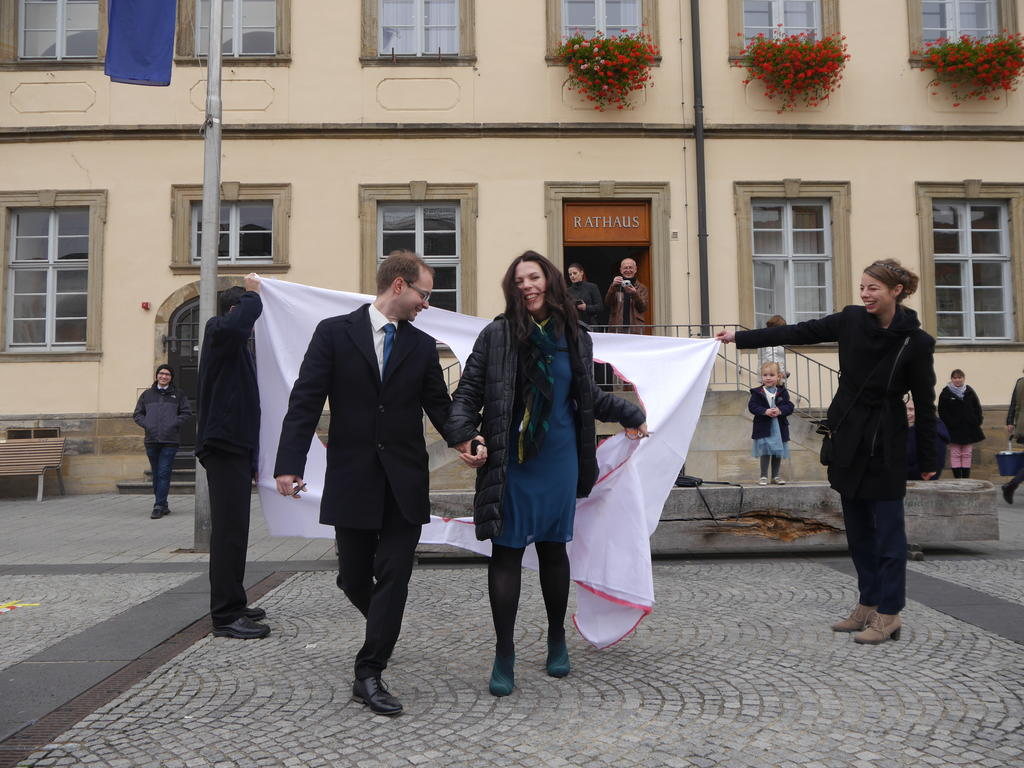
\includegraphics[width=\textwidth]{pic/kuchen.jpg}
\end{figure}


\begin{recipe}
[% 
    preparationtime = {\unit[30]{min}},
    bakingtime={\unit[80]{min}},
    bakingtemperature={\protect\bakingtemperature{
        fanoven=\unit[170]{\textcelcius}}},
    source = {Lieblingskuchen von Linus}
]
{Bierkuchen}
        
    
    \ingredients{%
        100g	& Butter \\	
		250g    & Zucker \\
		2		& Eier \\
		1 TL	& Zimt \\
		1 TL	& Nelken \\
		100g 	& Zitronat\\
		100g 	& Orangeat\\
		250g	& Sultaninen\\
		375g	& Mehl\\
		\unitfrac{1}{2} Seidla & Bier, nicht zu hopfig \\
		1 TL	& Natron\\
    }
    
    \preparation{%
    \newline
       \step Butten weich werden lassen, Natron im Bier aufl"osen und zusammen mit den anderen Zutaten gut verr"uhren. Nebenbei vom restlichen Bier trinken -- R"uhren ist nunmal anstrengend.
       \step Masse in eine gro\ss e, unter Umst"anden gefettete Kastenkuchenform einf"ullen.
       \step Backen. Dauert lange, aber man kann sich ja noch ein weiteres Bier aufmachen.
       \step Nach dem Backen ausk"uhlen lassen und mit Puderzucker bestreuen.
    }
    \suggestion{Es bietet sich an den Kuchen "uber Nacht stehen zu lassen, damit er sein Aroma optimal entfalten kann.}

    \hint{%
       Der Kuchen b"ackt zwar sehr lange, daf"ur ist er aber auch "uber eine Woche lang haltbar -- sofern er so "uberhaupt lange "uberlebt. 
    }
    
\end{recipe}

\end{otherlanguage}

\clearpage
~\thispagestyle{empty}
% Last page
\clearpage
\thispagestyle{empty}
~
\vfill
\begin{center}
\begin{tikzpicture}[scale=1.5]
\fill (0,0) -- (-0.2, 0.1) -- (-4, 0) -- (-0.2, -0.1) -- cycle;
\fill (0,0) -- (0.2, 0.1) -- (4, 0) -- (0.2, -0.1) -- cycle;
\fill (0,0) circle (0.1);
\end{tikzpicture}
\end{center}


    Eine hochzeitliche Rezeptesammlung -- Gerichte die wir G"aste lecker finden! Wir hoffen ihr findet die eine oder andere Anregung und denkt beim Kochen und Genießen an uns und das wundersch"one Fest.
    
    Wenn ihr mal ausgeschlafen habt könnt ihr unsere ganzen pull-requests unter \url{https://github.com/whatever4711/cookbook} annehmen.
\end{document} 